\documentclass[11pt,a4paper]{article}
\usepackage[margin=22mm]{geometry}
\usepackage{amsmath,amssymb,booktabs,graphicx,url,longtable}
\usepackage[hidelinks]{hyperref}
\usepackage{times}
\renewcommand{\thesection}{S\arabic{section}}
\renewcommand{\thetable}{S\arabic{table}}
\renewcommand{\thefigure}{S\arabic{figure}}
\renewcommand{\theequation}{S\arabic{equation}}
\title{Supplementary material\\\large Selective mask readout calibration through predicted correction benefit}
\author{Author information supplied separately}
\date{}
\makeatletter
\let\tableinput\@@input
\makeatother
\begin{document}
\maketitle

\section{Exact interpretation of the readout intervention}
The segmenter returns shared prototypes $P$, candidate coefficients $c_i$, predicted boxes, class IDs, and confidence scores. The experiment freezes all of these quantities within each model's candidate bank. The continuous mask is formed by coefficient--prototype multiplication, bilinear upsampling to the letterboxed input grid, and cropping with the original predicted box. Thresholding happens on that input grid. Export to the original image subsequently scales the binary mask and casts it to unsigned bytes, following the selected Ultralytics 8.4.100 utilities. It does not first resize the continuous logits to the original image and then threshold them.

The baseline threshold is zero in logit units. The trial threshold is $0.75/(1+(A/2304)^2)$, where $A$ is the original-image area of the exported baseline mask, in pixels. This is not a probability threshold of 0.75. A zero logit threshold corresponds to sigmoid probability 0.5 before the export operation. Thresholding a cropped logit tensor at nonnegative values keeps its zero-filled exterior off. All mask variants retain the predicted box; no expanded or ground-truth box is substituted.

The baseline and trial masks satisfy $M^t\subseteq M^0$ under this monotone export. Define the effective trial $M^1=M^t$ for nonempty trials and $M^1=M^0$ otherwise. The effective trial is still a subset of the baseline, with equality in the fallback case. The response gate chooses between these two masks and cannot add foreground. A baseline-exported empty mask remains outside the prediction set. Baseline nonempty predictions cannot disappear under the response gate.

The term ``tightening'' describes a thresholded response operation. It is not a morphological erosion with a fixed spatial radius. A threshold change may remove a weak interior component, enlarge an internal hole, or delete a thin object part as well as move an external contour. ``Boundary-only'' in the factorial experiment means changing the mask while preserving candidate identity and count; it does not mean changing only a narrow boundary band.

\section{IoU change and the decision objective}
\subsection{Proof of the removal condition}
Let $g>0$ be GT area, $T$ the baseline true-positive area, and $F$ its false-positive area. Let $u\in[0,T]$ and $v\in[0,F]$ be the corresponding removed areas. Both denominators below are positive:
\begin{align}
 J'-J
 &=\frac{T-u}{g+F-v}-\frac{T}{g+F}\\
 &=\frac{(T-u)(g+F)-T(g+F-v)}{(g+F-v)(g+F)}\\
 &=\frac{Tv-(g+F)u}{(g+F-v)(g+F)}.
\end{align}
Its sign is therefore the sign of $Tv-(g+F)u$. This is exact set algebra, not a novel bound on the neural network. If only false positives are removed and $T>0$, IoU increases. If only true positives are removed, it decreases. If $T=0$, deleting pixels cannot produce positive IoU because no true foreground is added. Empty-mask restoration yields zero change. Pixel purity alone cannot determine the sign because it does not retain the coverage term.

\subsection{What is and is not optimized}
The supervised target is the continuous change $\Delta=J(M^1,G)-J(M^0,G)$. For a population squared-error objective, the optimal unrestricted predictor is $f(x)=\mathbb{E}[\Delta\mid x]$. Choosing the trial when $f(x)>0$ maximizes expected per-instance IoU between these two actions, conditional on the supplied features. The fitted finite tree ensemble only approximates that quantity. No theorem in this work guarantees its prediction sign is correct or transfers without distribution shift.

AP additionally depends on category-wise confidence ordering, mask matching at multiple thresholds, false detections, and interpolation of the precision--recall curve. A conditional-mean IoU decision is consequently not an AP-optimal policy. Fixed-slot R75 is also a thresholded objective, different from continuous IoU. This distinction explains why area/shape/response ordering may differ across metrics. The paper reports empirical AP and transition counts rather than inferring one from the other.

\section{Calibration data, matching, and feature definitions}
\subsection{Data split}
Python's \texttt{random.Random(20260915).shuffle} is applied to train2017 image records sorted by image ID. The first 2,000 records are selected without class, failure, size, or crowding filtering. The first 1,500 are the gate-fit split; the remaining 500 are the gate/global-threshold selection split. All original annotations for each image are retained. This produces 10,288 matched ordinary GT training slots from 1,486 of the 1,500 fit images. Images without a matched slot contribute no regression target. The selection set contains 3,298 matched slots.

The final confirmation set is val2017 image IDs sorted numerically and sliced as \texttt{[500:5000]}. It contains 4,500 images and 32,831 non-crowd GT instances. The earlier 500-image development set is \texttt{val2017[:500]}, which must not be confused with the 500-image train2017 selection set. Validation was used in preceding exploratory diagnostics; this is not a new blind sample. The final fitted gate parameters are fixed before the reported 4,500-image application. The s transfer changes the pretrained weight scale without changing this gate or its decision rule.

\subsection{Instance identity and fixed-slot matching}
Ground truth is obtained from original COCO annotation IDs with \texttt{annToRLE}; polygons within one annotation are combined according to the official mask API. COCO category IDs are restored when exporting the model's contiguous class IDs. Standard COCOeval handles crowd annotations normally. The separate mechanism diagnostic uses non-crowd annotations only.

For each image, baseline predictions are ordered by descending confidence using a stable sort. Baseline-exported empty masks are skipped. A prediction is matched to the available ordinary GT of the same class with maximum box IoU, provided IoU is at least 0.50. The matched GT is then removed from the available set. GT candidates are considered in sorted index order for deterministic ties. This matching is not an oracle assignment that maximizes total mask IoU. It remains fixed across calibration variants and may differ between the m and s models.

There are 30,426 matched m slots and 2,405 unmatched GT; for s, 29,480 and 3,351. The R75 denominator is 32,831 for either model. Unmatched GT contribute failures and cannot be repaired by changing existing masks. Correct baseline counts are 19,065 (m) and 17,430 (s). The regression is fitted on matched slots but applied to every nonempty baseline candidate, including unmatched detections; that difference in population is an explicit limitation.

\subsection{Five features}
Let $A=|M^0|$ on the original image. Let $w,h$ be the width and height of the smallest axis-aligned rectangle containing the original-image binary mask, using inclusive pixel extents. Let $a$ be baseline foreground area on the input grid and $p_4$ its four-connected perimeter, counting differing horizontal/vertical neighboring pixels and positive pixels on the grid boundary. The features are
\begin{align}
 x_1&=\log(1+A),\\
 x_2&=\log\!\left(1+\frac{\max(w,h)}{\max(\min(w,h),1)}\right),\\
 x_3&=\frac{A}{\max(wh,1)},\\
 x_4&=\log\!\left(1+\frac{p_4^2}{4\pi\max(a,1)}\right),\\
 x_5&=\frac{A-|M^t|}{\max(A,1)}.
\end{align}
The first gate uses $x_1$, the second $x_1$--$x_4$, and the final response gate all five. The raw trial area is used in $x_5$ even when a newly empty mask is restored; its training target is then zero. The deployment implementation uses float32 perimeter/compactness arithmetic before converting the feature array to float64 for tree prediction, matching the candidate-bank representation. Features contain no class or score.

\subsection{Fit and selection settings}
All regressors use scikit-learn histogram gradient boosting with squared error, 100 iterations, learning rate 0.05, maximum seven leaves, minimum leaf size 80, $L_2=1$, and disabled early stopping. The regressor seed is 20260915. No separate gate cutoff is fitted: positive predicted gain activates the trial. Table~\ref{tab:selection} reports selection AP. The global grid additionally includes 0, 0.5, 0.75 and 1; the selected value is 0.25, with ties favoring a smaller threshold.

\begin{table}[htbp]\centering
\caption{COCO Mask AP on the 500-image train2017 selection set. These are selection results, not final validation results.}\label{tab:selection}
\begin{tabular}{lr}\toprule Rule & AP\\\midrule
\tableinput{tables/selection.tex}
\bottomrule\end{tabular}
\end{table}

\section{Complete COCO metrics and filtering controls}
Tables~\ref{tab:allap} and \ref{tab:allar} give the official segmentation evaluator's twelve statistics. All metrics are on the 0--100 scale. The evaluator uses its default max-detection limits (1, 10, 100); the predictor's separate candidate limit is 300. Size-specific evaluation follows official COCO area handling. The input pipeline is the selected predictor/export pipeline, not a claim that every stage is identical to a published full \texttt{model.val} run.

\begin{table}[htbp]\centering\small
\caption{All AP statistics, 4,500-image validation confirmation.}\label{tab:allap}
\setlength{\tabcolsep}{4pt}
\begin{tabular}{llrrrrrr}\toprule Model & Readout & AP & AP$_{50}$ & AP$_{75}$ & AP$_S$ & AP$_M$ & AP$_L$\\\midrule
\tableinput{tables/full_ap.tex}
\bottomrule\end{tabular}\end{table}

\begin{table}[htbp]\centering\small
\caption{All AR statistics from COCOeval; these are not fixed-slot R75.}\label{tab:allar}
\setlength{\tabcolsep}{4pt}
\begin{tabular}{llrrrrrr}\toprule Model & Readout & AR$_1$ & AR$_{10}$ & AR$_{100}$ & AR$_S$ & AR$_M$ & AR$_L$\\\midrule
\tableinput{tables/full_ar.tex}
\bottomrule\end{tabular}\end{table}

For m, the baseline has 507,043 pre-export candidates, 77 of which have empty exported masks, leaving 506,966 predictions. Fixed smooth produces 998 additional empty outputs. Filtering-only drops these 998 outputs but uses baseline masks for the remainder. Boundary-only keeps all 506,966 baseline outputs, substitutes each available trial, and restores the baseline for newly empty trials. Table~\ref{tab:factorial} isolates these operations. The AP interaction is defined as $AP_{\rm both}-AP_{\rm boundary}-AP_{\rm filter}+AP_{\rm base}$. Its value is approximately 0.000033 points, so it is not an unexplained large interaction masked by rounding.

The m response gate calibrates 366,598 and retains 140,368 of the baseline's nonempty exports. The s baseline has 558,921 candidates and 43 empty baseline exports; its response gate retains a total of 558,878 nonempty predictions. AP is always recomputed from complete exported predictions with original category IDs and scores. No GT-dependent filtering is performed at evaluation.

\begin{table}[htbp]\centering
\caption{Factorial m-model control. Extra precision is shown only to distinguish the small filtering effect.}\label{tab:factorial}
\begin{tabular}{lrr}\toprule Operation & AP & $\Delta$AP\\\midrule
\tableinput{tables/factorial.tex}
\bottomrule\end{tabular}\end{table}

\section{Transitions, intervals, and conditional interpretation}
For each image $j$, let $n_j$ be its number of ordinary GT and $d_{j,k}$ the net repaired-minus-damaged count for rule $k$. The fixed-slot gain is $100\sum_jd_{j,k}/\sum_jn_j$. Bootstrap sampling draws 4,500 image indices with replacement, retaining every instance and all compared methods for each selected image. Each resample recomputes the denominator. We use 2,000 draws from NumPy's default random generator with seed 20260915 and percentile endpoints 2.5\% and 97.5\%. Comparing methods uses the same draws. These intervals quantify sampling variation of the fixed fitted rules; they do not capture calibration-fit variation or AP uncertainty.

\begin{table}[htbp]\centering
\caption{Paired differences in fixed-slot R75 (percentage points).}\label{tab:ci}
\begin{tabular}{llrr}\toprule Model & Comparison & Difference & 95\% interval\\\midrule
m & Response minus area & 0.302 & [0.183, 0.424]\\
m & Response minus fixed smooth & 0.076 & [$-0.018$, 0.169]\\
s & Response minus area & 0.305 & [0.188, 0.417]\\
s & Response minus fixed smooth & 0.168 & [0.070, 0.270]\\
\bottomrule\end{tabular}\end{table}

The high-coverage failure group is defined entirely from baseline matching and baseline mask measurements. All members fail at 0.75 by construction, so no initially correct instance can be damaged within this group. The group-specific repair percentage must therefore be accompanied by damage counts in the full matched population. Similarly, high purity after tightening is not sufficient evidence of correct segmentation: target coverage is reported alongside it. The selected m gate's mean coverage decreases from 0.9807 to 0.9645 in this group. The result is a more favorable trade-off, not proof of lossless recovery or perfect separation of neighboring instances.

\section{Illustrative development examples}
Figure~\ref{fig:examples} shows previously recorded development examples of the fixed smooth trial, before the learned gate is applied. Within each development transition group, the example is selected by median absolute IoU change, with image ID and annotation ID resolving ties. These three cases illustrate the intervention's opposing effects; they are not final-gate outputs or a new validation estimate.

The first object (image 54967, annotation 360620) changes from IoU 0.7040 to exactly 0.7500, while target coverage changes from 0.9888 to 0.9775. The second (image 3934, annotation 2155391) improves from 0.7352 to 0.7758 despite a coverage decrease from 0.9163 to 0.8522. The third (image 25603, annotation 2017204) is damaged: IoU decreases from 0.7753 to 0.7121 while purity increases from 0.9841 to 0.9923. This last case demonstrates why purity alone cannot validate tightening. Each figure row is an enlarged original-image crop; no image enhancement or synthetic content is used.

\begin{figure}[p]\centering
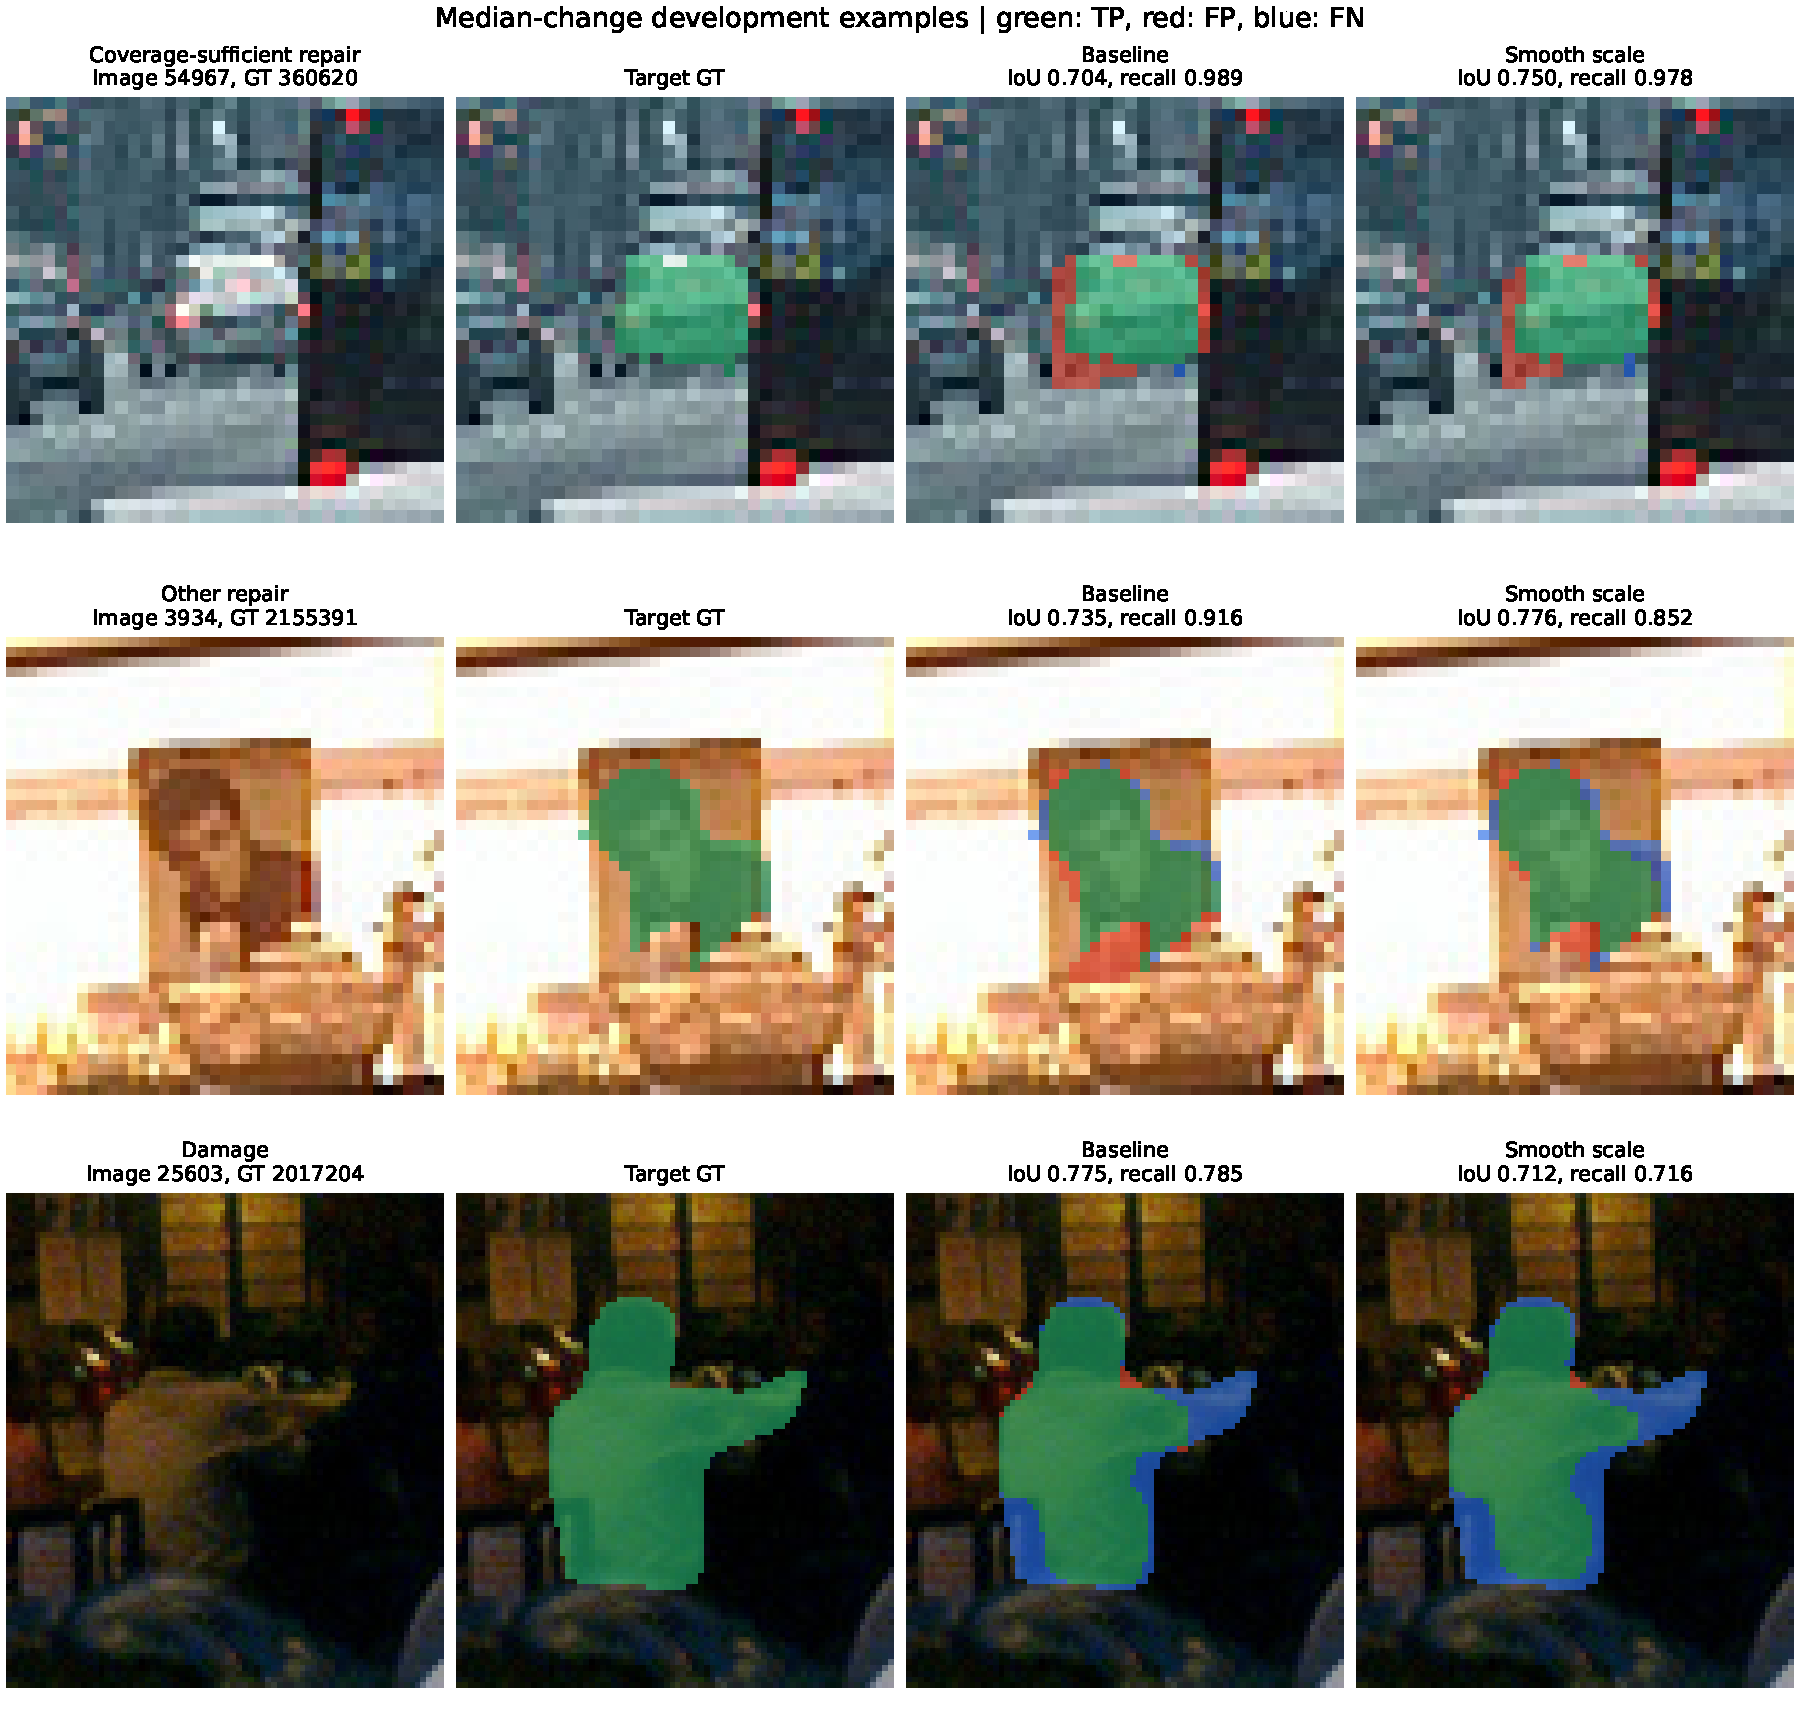
\includegraphics[width=\textwidth]{figures/development_examples.pdf}
\caption{Median-change examples from the 500-image val2017 development set, showing the fixed smooth trial. Green: true-positive pixels; red: false-positive pixels; blue: false-negative pixels relative to the target GT. Labels marked ``recall'' mean target coverage. These are diagnostic trial examples, not predictions of the final response gate.}\label{fig:examples}
\end{figure}

\section{Deployment and timing}
The inference adapter evaluates logits in chunks of 24 candidates, constructs baseline and trial exports, computes the five features, and applies the frozen tree ensemble on the CPU. Its output selects the input-grid baseline or trial mask before returning the normal predictor result. Newly empty trial exports use baseline masks. Float32 compactness computation is preserved because differing numerical precision can move a feature across a tree split.

Portable JSON tree representations were checked against the fitted joblib estimators on the 507,043-candidate m bank: all three gates produced zero maximum prediction difference and zero decision differences in that check. This avoids dependence on pickle compatibility between the fitting and inference machines. The real adapter was also checked against bank features and output masks on a three-image, 423-candidate smoke test; that test is limited interface verification, not full-dataset end-to-end validation.

Timing uses an RTX 4060 Laptop GPU with 8 GB VRAM, batch one, and FP32. Eight warm-up calls precede each block. Eighty evenly spaced images are evaluated in four rounds with rotated method ordering, giving 320 timed calls per method. Timings include preprocessing, forward inference, mask construction, feature movement, and tree prediction, and exclude disk I/O, initialization, warm-up, RLE export, and COCOeval. The official predictor's block means are 42.96, 35.62, 35.02, and 35.46 ms; the elevated first block makes the overall mean an imperfect steady-state estimate. The response gate block means are 57.31, 58.33, 57.06, and 56.80 ms. The comparison to the similarly chunked fixed rule is consequently informative as well.

\begin{table}[htbp]\centering
\caption{Measured latency distribution (ms), including gate work.}\label{tab:speed}
\begin{tabular}{lrrr}\toprule Implementation & Mean & Median & P95\\\midrule
\tableinput{tables/latency.tex}
\bottomrule\end{tabular}\end{table}

\section{Reproducibility package and evidence scope}
The accompanying manuscript directory contains the table-generation script, machine-readable table values, vector figures, and an evidence-source map referencing the completed experimental runs. The local reproducibility directory includes the fixed gate JSONs, relevant decoder and fitting scripts, the calibration split, and the validation image IDs. COCO images and pretrained weights are obtained separately from their original providers. No public repository address is asserted until the authors choose a release destination.

All main results use the one-to-one branch. Historical results using other decoder/export orders, one-to-many inference, partial image subsets, or coefficient-orthogonality training do not enter the reported tables. Table generation reads completed JSON results and does not rerun or refit the segmenter. The paper's conclusions are limited to the evaluated rules, dataset subset, and two pretrained scales. The supplementary material makes no additional cross-dataset, blind-test, or repeated-training claim.
\end{document}
